\documentclass[
    hyperref={hidelinks=true}
]{beamer}

\usepackage{listings}
\usepackage{mhchem}
\usepackage{xcolor}
\usepackage{chemstyle}
\usepackage{tikz}
\usepackage{xstring}
\usepackage{mathtools}
\usepackage{amsmath}
\usepackage{physics}
\usepackage{tikz-3dplot}
\usepackage{ifthen}
\usepackage{circuitikz}
\usepackage{pgfplots}

\usetikzlibrary{math}
\usetikzlibrary{fit,positioning}

\let\Re\relax
\DeclareMathOperator{\Re}{Re}
\let\Im\relax
\DeclareMathOperator{\Im}{Im}

\definecolor{codegreen}{rgb}{0,0.6,0}
\definecolor{codegray}{rgb}{0.5,0.5,0.5}
\definecolor{codepurple}{rgb}{0.58,0,0.82}
\definecolor{backcolour}{rgb}{0.95,0.95,0.92}
\definecolor{comment-color}{rgb}{132, 156, 138}

\lstdefinestyle{mystyle}{
    backgroundcolor=\color{backcolour},  
    commentstyle=\color{codegreen},
    keywordstyle=\color{magenta},
    numberstyle=\tiny\color{codegray},
    stringstyle=\color{codepurple},
    basicstyle=\ttfamily\footnotesize,
    breakatwhitespace=false,        
    breaklines=true,                
    captionpos=b,                    
    keepspaces=true,                
    numbers=left,                    
    numbersep=5pt,                  
    showspaces=false,                
    showstringspaces=false,
    showtabs=false,                  
    tabsize=2
}

\lstset{style=mystyle}

\title{{\LaTeX} for CDT chemists}
\author{Richard Cox}
\institute{TECS CDT}
\date{2023}

\newcommand{\csubtitle}[1]{\textbf{#1} \\}


\begin{document}

\frame{\titlepage}


\begin{frame}
\frametitle{Why use \LaTeX?}
From \href{https://www.overleaf.com/learn/latex/Learn_LaTeX_in_30_minutes}{overleaf:} \pause
\begin{itemize}
    \item support for typesetting extremely complex mathematics, tables and technical content for the physical sciences \pause
    \item facilities for footnotes, cross-referencing and management of bibliographies \pause
    \item ease of producing complicated, or tedious, document elements such as indexes, glossaries, table of contents, lists of figures \pause
    \item being highly customizable for bespoke document production due to its intrinsic programmability and extensibility through thousands of free add-on packages \pause
    \item  great deal of control over the production of documents which are typeset to extremely high standards \pause
    \item separation of document content from document style
\end{itemize}

\end{frame}


\begin{frame}
    \frametitle{Writing \LaTeX}
    Unlike other document-producing programs, {\LaTeX} is written in a plain text (.txt) file -- therefore, it is free and its compilers are open-source! \\ \pause
    Choose a good code editor. You can use:
    \begin{itemize}
        \item Notepad -- any editor will do, right? \pause
        \item {\TeX}maker, {\TeX}studio or {\TeX}works -- {\LaTeX}-specialised code editors \pause
        \item Visual studio code -- all-purpose, lightweight and highly customisable code editor -- \textbf{recommended for advanced users} \pause
        \item \url{overleaf.com} -- if VSCode is MS word, then overleaf is google docs. All your work is saved to the cloud -- \textbf{recommended for beginners}
    \end{itemize}
\end{frame}



\begin{frame}[fragile]
\frametitle{Setting up a {\LaTeX} document}

\begin{lstlisting}
\documentclass{article}

\begin{document}
    Hello world!

\end{document}
\end{lstlisting}

\end{frame}


\begin{frame}[fragile]
    \frametitle{Setting up a {\LaTeX} document}
   
    \begin{lstlisting}
\documentclass[a4paper,12pt]{article}
\title{LaTeX test}
\author{Richard Cox}
\date{}

\begin{document}
    \maketitle

    \section{Introduction}
        Hello world!

        \subsection{}

        Some text in a subsection

\end{document}
    \end{lstlisting}
   
\end{frame}


\begin{frame}[fragile]
    \frametitle{Setting up a {\LaTeX} document}
   
    \begin{lstlisting}
\documentclass[a4paper,12pt,twocolumn]{article}
\title{LaTeX test}
\author{Richard Cox}
\date{}

\usepackage[left=20mm, right=20mm, top=20mm, bottom=20mm]
\usepackage{lipsum}

\begin{document}
    \maketitle

    \section{Introduction}
        \lipsum{1}

        \subsection{A subsection}

        \lipsum{1-3}

\end{document}
    \end{lstlisting}
   
\end{frame}




\begin{frame}[fragile]
\frametitle{The preamble}
Works similarly to a python script:

\begin{lstlisting}
import seaborn as sns
import pandas as pd

tips = pd.read_csv("https://milliams.com/courses/data_analysis_python/tips.csv")
sns.catplot(data=tips, x="day", y="bill_per_person", order=["Thur", "Fri", "Sat", "Sun"], kind="box")
\end{lstlisting}

Think of this as where you do general page set-up, creating commands, etc. \\
Must have the packages you want to invoke \textbf{BEFORE} the code \\
What's a better place to put it than before \verb|\begin{document}|? \\

\end{frame}



\begin{frame}[fragile]
    \frametitle{Using packages}
    \begin{itemize}
    \item Similarly to python libraries, packages are snippets of code made by other people that do things
    \item Use the command \verb|\usepackage[]{}| to load a package
    \item \verb|{}| lets you specify the arguament; in this case, the package
    \item \verb|[]| lets you include options -- detailed in the \textit{package documentation}
    \item adding \verb|*| to most commands means they won't be numbered or won't appear in the table of contents
    \end{itemize} \pause
    Example:
    \begin{lstlisting}
\usepackage{mhchem} % Easy chemistry formatting
\usepackage{graphicx} % Including images in LaTeX
\usepackage[margin=1in]{geometry} % Better page sizing
    \end{lstlisting}
\end{frame}



\begin{frame}[fragile]
    \frametitle{The main body}
    All displayed text is written in an enviroment:
    \begin{lstlisting}
\begin{env}

    Some text
    \some-commands

\end{env}
    \end{lstlisting}
    The visual part of the whole document is in the \verb|document| environment, between \verb|\begin{document}| and \verb|\end{document}|

\end{frame}



\begin{frame}[fragile]
\frametitle{Useful text commands}
\begin{itemize}
\item \textbf{Bold text}: \verb|\textbf{}|
\item \textit{Italicised text}: \verb|\textit{}|
\item \underline{Underlined text}: \verb|\underline{}|
\item \textcolor{codegray}{Commented text}: \verb|Some commented text|
\item \textsuperscript{Superscript text}: \verb|\textsuperscript{}|
\item \textsubscript{Subscript text}: \verb|\textsubscript{}| \pause
\item Adding a label to a figure, table, scheme or equation: \verb|\label{}|
\item Cross-referencing a figure, table, scheme or equation: \verb|\ref{}| \pause
\item Linebreak: \verb|\\| or \verb|\linebreak|
\item pagebreak: \verb|\pagebreak|
\item Including other .tex files: \verb|\include{}| \pause
\item Adding a table of contents: \verb|\tableofcontents|
\item Adding to a table of content: \verb|\addcontentsline{toc}{section}|
\end{itemize}
\end{frame}





\begin{frame}[fragile]
\frametitle{Maths in \LaTeX}
\begin{itemize}
    \item For an inline maths environment, use \verb|$some maths$|
    \item For a displayed maths environment, use \verb|\begin{math}| and \verb|\end{math}|
    \item For equations, use \verb|\begin{equation}| and \verb|\end{equation}| (n.b. equations are numbered automatically like figures and tables!)
\end{itemize} \pause
Inside maths environments, treat it like an inline maths calculator:
\begin{itemize}
    \item For subscript, use \verb|a_{n}| = $a_{n}$
    \item For superscript, use \verb|a^{n}| = $a^{n}$
    \item For fractions, use \verb|\frac{numerator}{denominator}|
    \item For greek letters, use \verb|\greek-letter| (e.g. \verb|$\alpha$| = $\alpha$)
\end{itemize}
\end{frame}





\begin{frame}[fragile]
    \frametitle{Making tables}
    Use the \verb|table| and \verb|tabular| environments:
\begin{lstlisting}
\begin{table}[float]
    \begin{tabular}{l }
        Column 1 & Column 2 & column 3 \\
        Some more & Some more & More data \\
    \end{tabular}
    \caption{}
    \label{}
\end{table}

\end{lstlisting} \pause

Give the number of columns after tabular:
\begin{itemize}
    \item left: \verb|l|
    \item right: \verb|r|
    \item center: \verb|c|
    \item custom width: \verb|p{xcm}|
\end{itemize}

There are some great online tools to quickly generate table environments from excel, like \url{https://www.tablesgenerator.com}!

\end{frame}






\begin{frame}[fragile]
\frametitle{Using pictures with \href{https://anorien.csc.warwick.ac.uk/mirrors/CTAN/macros/latex/required/graphics/grfguide.pdf}{graphicx}}
Use the figure environment:
\begin{lstlisting}
\usepackage{graphicx}
...
\begin{figure}[floats]
    \centering
    \includegraphics[sizing]{PATH_TO_FIGURE}
    \caption{}
    \label{}
\end{figure}
\end{lstlisting} \pause
Floats control positioning on the page
\begin{itemize}
    \item t = top of page
    \item b = bottom of page
    \item h = relative in the text
    \item H (with \verb|float| package) = relative in text, overriding \LaTeX placement algorithm
\end{itemize}
sizing options:
\begin{itemize}
    \item \verb|width = 0.8\linewidth|
    \item \verb|scale = 0.8|
\end{itemize}


\end{frame}



\begin{frame}[fragile]
    \frametitle{Practice - adding images with \href{https://anorien.csc.warwick.ac.uk/mirrors/CTAN/macros/latex/required/graphics/grfguide.pdf}{graphicx}}
    Draw out the Chan-Lam reaction from the DoE experiment, and add it to the document
\end{frame}




\begin{frame}[fragile]
    \frametitle{Using minipages}
    Can separate page into sections, and have two figures on the same line
    \begin{lstlisting}
\usepackage[labelfont=bf]{caption,subcaption}
...
\begin{figure}[h]
    \centering



    \caption{}
    \label{}
\end{figure}
    \end{lstlisting}
\end{frame}


\begin{frame}[fragile]
    \frametitle{Using minipages}
    \begin{lstlisting}
\usepackage[labelfont=bf]{caption,subcaption}
...
\begin{figure}[h]
    \centering
    \begin{minipage}{0.49\linewidth}
        \includegraphics{}
        \subcaption{}
    \end{minipage}
    \begin{minipage}{0.49\linewidth}
        \includegraphics{}
        \subcaption{}
    \end{minipage}
    \caption{}
    \label{}
\end{figure}
    \end{lstlisting}
\end{frame}





\begin{frame}
    \frametitle{Images with Ti\textit{k}Z}
    Ti\textit{k}Z provides libraries for making graphics in {\LaTeX} \\ \pause

    \begin{columns}[t]
    \column{0.3\textwidth}
    \centering
    \usetikzlibrary{math}

\scalebox{0.4}{%
    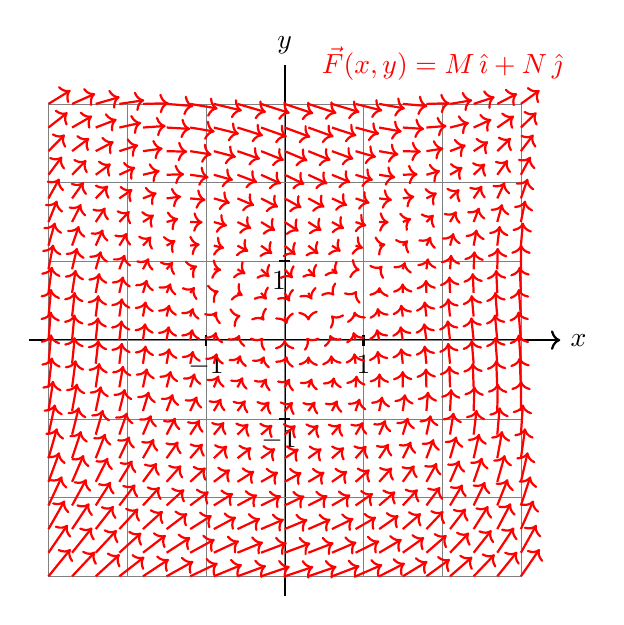
\begin{tikzpicture}
        % Components of the vector field
        \tikzmath{function equis(\x,\y) {return (\y*\y-0.25*\x);};}
        \tikzmath{function ye(\x,\y) {return \x*\x-\y;};}
        \tikzmath{function zeta(\x,\y) {return \x+\y;};}	
        \tikzmath{function magnitud(\x,\y) {return sqrt(\x*\x+\y*\y);};} % magnitude of the vector at (x, y, z)	
        %	
        \pgfmathsetmacro{\dominio}{3.0}	% domain for computation 
        \pgfmathsetmacro{\step}{\dominio/10.0} % step size
        \pgfmathsetmacro{\max}{\dominio}
        \pgfmathsetmacro{\xi}{-\dominio}
        \pgfmathsetmacro{\xf}{\dominio}
        \pgfmathsetmacro{\xs}{\xi+\step}
        \pgfmathsetmacro{\yi}{-\dominio}
        \pgfmathsetmacro{\yf}{\dominio}
        \pgfmathsetmacro{\ys}{\yi+\step}
        % length of coordinate axis
        \pgfmathsetmacro{\ejex}{\dominio+0.50}
        \pgfmathsetmacro{\ejez}{\dominio+0.50}
        % Coordinate axis
        \draw[thick,->] (\xi-0.25,0) -- (\xf+0.5,0) node[right] {$x$}; % Eje x
        \draw[thick] (0,\yi-0.25,0) -- (0,\yf+0.5) node[above] {$y$}; % Eje y
        \draw[help lines] (\xi,\yi) grid (\xf,\yf);
        \foreach \x in {-1,1}
            \draw[thick] (\x,2pt) -- (\x,-2pt) node [below] {$\x$};
        \foreach \y in {-1,1}
            \draw[thick] (2pt,\y) -- (-2pt,\y) node [below] {$\y$};
        % The vector field
        \foreach \x in {\xi,\xs,...,\xf}{
            \foreach \y in {\yi,\ys,...,\yf}{
                % Components of the vector at (\x,\y)
                \pgfmathsetmacro{\vx}{0.125*equis(\x,\y)/(magnitud(\x,\y)+0.1)}
                \pgfmathsetmacro{\vy}{0.125*ye(\x,\y)/(magnitud(\x,\y)+0.1)}
                \draw[red,thick,->] (\x,\y) -- (\x+\vx,\y+\vy);
            }
        }
        \node[red,above,shift={(-1,5pt)}] at (\xf,\yf) {$\vec{F}(x,y) = M\,\hat{\imath} + N\,\hat{\jmath}$};
        %
    \end{tikzpicture}
} \pause
    % Variational autoencoder architecture. The earliest type of generative machine learning model.
% Inspired by https://towardsdatascience.com/intuitively-understanding-variational-autoencoders-1bfe67eb5daf.




\usetikzlibrary{fit,positioning}

\newcommand\drawNodes[2]{
  % #1 (str): namespace
  % #2 (list[list[str]]): list of labels to print in the node of each neuron
  \foreach \neurons [count=\lyrIdx] in #2 {
    \StrCount{\neurons}{,}[\lyrLength] % use xstring package to save each layer size into \lyrLength macro
    \foreach \n [count=\nIdx] in \neurons
      \node[neuron] (#1-\lyrIdx-\nIdx) at (2*\lyrIdx, \lyrLength/2-1.4*\nIdx) {\n};
  }
}

\newcommand\denselyConnectNodes[2]{
  % #1 (str): namespace
  % #2 (list[int]): number of nodes in each layer
  \foreach \n [count=\lyrIdx, remember=\lyrIdx as \previdx, remember=\n as \prevn] in #2 {
    \foreach \y in {1,...,\n} {
      \ifnum \lyrIdx > 1
        \foreach \x in {1,...,\prevn}
          \draw[->] (#1-\previdx-\x) -- (#1-\lyrIdx-\y);
      \fi
    }
  }
}

\scalebox{0.2}{%
\begin{tikzpicture}[
    shorten >=1pt, shorten <=1pt,
    neuron/.style={circle, draw, minimum size=4ex, thick},
    legend/.style={font=\large\bfseries},
  ]

  % encoder
  \drawNodes{encoder}{{{,,,,}, {,,,}, {,,}}}
  \denselyConnectNodes{encoder}{{5, 4, 3}}

  % decoder
  \begin{scope}[xshift=11cm]
    \drawNodes{decoder}{{{,,}, {,,,}, {,,,,}}}
    \denselyConnectNodes{decoder}{{3, 4, 5}}
  \end{scope}

  % mu, sigma, sample nodes
  \foreach \idx in {1,...,3} {
      \coordinate[neuron, right=2 of encoder-3-2, yshift=\idx cm,, fill=yellow, fill opacity=0.2] (mu-\idx);
      \coordinate[neuron, right=2 of encoder-3-2, yshift=-\idx cm, fill=blue, fill opacity=0.1] (sigma-\idx);
      \coordinate[neuron, right=4 of encoder-3-2, yshift=\idx cm-2cm, fill=green, fill opacity=0.1] (sample-\idx);
    }

  % mu, sigma, sample boxes
  \node [label=$\mu$, fit=(mu-1) (mu-3), draw, fill=yellow, opacity=0.45] (mu) {};
  \node [label=$\sigma$, fit=(sigma-1) (sigma-3), draw, fill=blue, opacity=0.3] (sigma) {};
  \node [label=sample, fit=(sample-1) (sample-3), draw, fill=green, opacity=0.3] (sample) {};

  % mu, sigma, sample connections
  \draw[->] (mu.east) edge (sample.west) (sigma.east) -- (sample.west);
  \foreach \a in {1,2,3}
  \foreach \b in {1,2,3} {
      \draw[->] (encoder-3-\a) -- (mu-\b);
      \draw[->] (encoder-3-\a) -- (sigma-\b);
      \draw[->] (sample-\a) -- (decoder-1-\b);
    }

  % input + output labels
  \foreach \idx in {1,...,5} {
      \node[left=0 of encoder-1-\idx] {$x_\idx$};
      \node[right=0 of decoder-3-\idx] {$\hat x_\idx$};
    }
  \node[above=0.1 of encoder-1-1] {input};
  \node[above=0.1 of decoder-3-1] {output};

\end{tikzpicture}
} \pause
    \column{0.3\textwidth}
    \centering
    \pgfmathdeclarerandomlist{colors}{{red!80}{teal}{blue!80}{orange}{blue!20}}

\scalebox{0.2}{%
\begin{tikzpicture}
  \foreach \i in {1,...,12} {
      \foreach \j in {1,...,4} {
          \foreach \k in {1,...,4} {
              \pgfmathrandomitem{\randColor}{colors}
              \shade[ball color=\randColor] (-\i+0.3*\j, -0.2*\j+1.2*\k) circle(0.3);
            }
          \foreach \k in {1,...,3} {
              \pgfmathrandomitem{\randColor}{colors}
              \shade[ball color=\randColor] (-\i+0.5+0.3*\j, -0.2*\j+1.2*\k+0.6) circle(0.3);
            }
        }
    }
  \foreach \el/\color [count=\n] in {Al/red!80, Co/blue!80, Cr/teal, Fe/orange, Ni/blue!20} {
      \shade[ball color=\color] (2, 5.5-\n) circle(0.3) node[right=1em] {\el};
    }
\end{tikzpicture}
} \pause
    \colorlet{myblue}{black!40!blue}
\colorlet{myred}{black!40!red}
\colorlet{vcol}{green!50!black}
\colorlet{Ecol}{orange!90!black}
\colorlet{EVcol}{orange!80!black!60}
\colorlet{Bcol}{violet!90}






\scalebox{0.3}{%
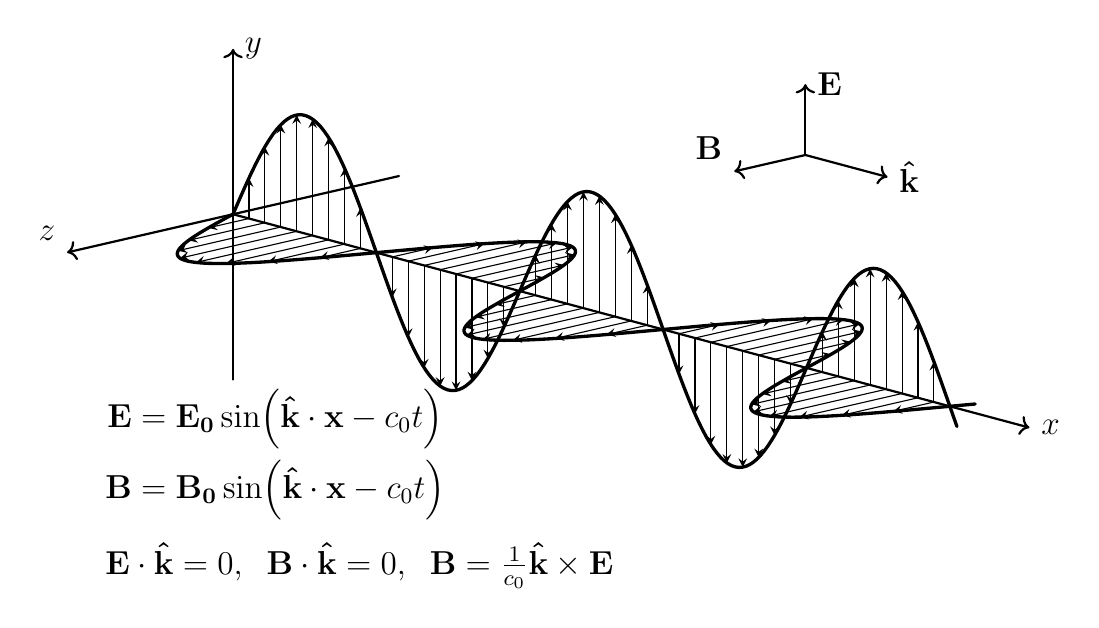
\begin{tikzpicture}[x=(-15:1.2), y=(90:1.0), z=(-150:1.0),
    line cap=round, line join=round,
    axis/.style={black, thick,->},
    vector/.style={>=stealth,->}]
\large
\def\A{1.5}
\def\nNodes{5} % use even number
\def\nVectorsPerNode{8}
\def\N{\nNodes*40}
\def\xmax{\nNodes*pi/2*1.01}
\pgfmathsetmacro\nVectors{(\nVectorsPerNode+1)*\nNodes}

\def\vE{\mathbf{E}}
\def\vB{\mathbf{B}}
\def\vk{\mathbf{\hat{k}}}

% MAIN AXES
\draw[axis] (0,0,0) -- ++(\xmax*1.1,0,0) node[right] {$x$};
\draw[axis] (0,-\A*1.4,0) -- (0,\A*1.4,0) node[right] {$y$};
\draw[axis] (0,0,-\A*1.4) -- (0,0,\A*1.4) node[above left] {$z$};

% SMALL AXES
\def\xOffset{{(\nNodes-2)*pi/2}}
\def\yOffset{\A*1.2}
\def\zOffset{\A*1.2}
\draw[axis] (\xOffset,\yOffset,-\zOffset) -- ++(\A*0.6,0,0) node[right] {$\vk$};
\draw[axis] (\xOffset,\yOffset,-\zOffset) -- ++(0,\A*0.6,0) node[right] {$\vE$};
\draw[axis] (\xOffset,\yOffset,-\zOffset) -- ++(0,0,\A*0.6) node[above left] {$\vB$};

% equation
\node[above right] at (\xOffset,-0.5*\yOffset,4*\zOffset)
{$\begin{aligned}
\vE &= \mathbf{E_0}\sin(\vk\cdot\mathbf{x}-c_0t)\\
\vB &= \mathbf{B_0}\sin(\vk\cdot\mathbf{x}-c_0t)\\
\end{aligned}$};
\node[below right] at (\xOffset,-0.5*\yOffset,4*\zOffset)
{$\vE\cdot\vk = 0,\;\; \vB\cdot\vk = 0,\;\; \vB = \frac{1}{c_0}\vk\times\vE$};

% waves
\draw[very thick,variable=\t,domain=0:\nNodes*pi/2*1.01,samples=\N]
plot (\t,{\A*sin(\t*360/pi)},0);
\draw[very thick,variable=\t,domain=0:\nNodes*pi/2*1.01,samples=\N]
plot (\t,0,{\A*sin(\t*360/pi)});

% draw vectors
\foreach \k [evaluate={\t=\k*pi/2/(\nVectorsPerNode+1);
         \angle=\k*90/(\nVectorsPerNode+1);
         \c=(mod(\angle,90)!=0);}]
in {1,...,\nVectors}{
\if\c1
\draw[vector] (\t,0,0) -- ++(0,{\A*sin(2*\angle)},0);
\draw[vector] (\t,0,0) -- ++(0,0,{\A*sin(2*\angle)});
\fi
}

\end{tikzpicture}
} \pause
    \column{0.3\textwidth}
    \centering
    
\pgfplotsset{compat=newest}




\scalebox{0.4}{%
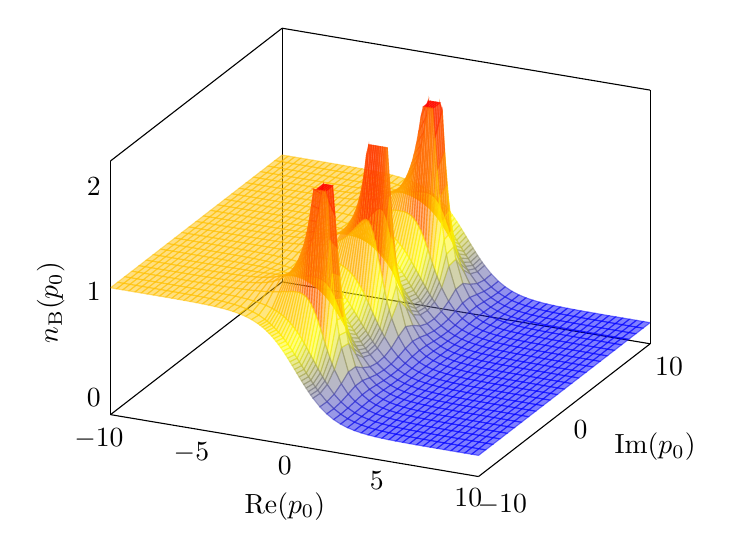
\begin{tikzpicture}
    \begin{axis}[
        xlabel=$\Re(p_0)$,
        ylabel=$\Im(p_0)$,
        zlabel=$n_\text{B}(p_0)$,
        x label style={at={(0.35, 0)}},
        y label style={at={(0.95, 0.15)}},
        shader=flat,
        tickwidth=0pt
      ]
  
      \def\nB{(e^(2*x) - 2*e^x*cos(deg(y)) + 1)^(-1/2)}
  
      \addplot3[surf, opacity=0.5, domain=1:10, y domain=-10:10]{\nB};
  
      \addplot3[surf, opacity=0.5, domain=-10:-2, y domain=-10:10]{\nB};
  
      \addplot3[surf, opacity=0.5, domain=-2:1, y domain=-10:10, restrict z to domain*=0:2]{\nB};
  
    \end{axis}
  \end{tikzpicture}
} \pause
    % Tikz Library
\usetikzlibrary{calc}

% Bipoles Specifications
\ctikzset{bipoles/thickness=1.2, label distance=1mm, voltage shift = 1}

% Arrows Above Compenents
% Source: https://tex.stackexchange.com/questions/574576/circuitikz-straight-voltage-arrows-with-fixed-length
\newcommand{\fixedvlen}[3][0.4cm]{% [semilength]{node}{label}
    % get the center of the standard arrow
    \coordinate (#2-Vcenter) at ($(#2-Vfrom)!0.5!(#2-Vto)$);
    % draw an arrow of a fixed size around that center and on the same line
    \draw[-{Triangle[round,open]}] ($(#2-Vcenter)!#1!(#2-Vfrom)$) -- ($(#2-Vcenter)!#1!(#2-Vto)$);
    % position the label as it where if standard voltages were used
    \node[ anchor=\ctikzgetanchor{#2}{Vlab}] at (#2-Vlab) {#3};
}
\newcommand{\fixedvlendashed}[3][0.75cm]{% [semilength]{node}{label}
    % get the center of the standard arrow
    \coordinate (#2-Vcenter) at ($(#2-Vfrom)!0.5!(#2-Vto)$);
    % draw an arrow of a fixed size around that center and on the same line
    \draw[dashed,-{Triangle[round,open]}] ($(#2-Vcenter)!#1!(#2-Vfrom)$) -- ($(#2-Vcenter)!#1!(#2-Vto)$);
    % position the label as it where if standard voltages were used
    \node[ anchor=\ctikzgetanchor{#2}{Vlab}] at (#2-Vlab) {#3};
}

\scalebox{0.3}{%
	\begin{circuitikz}
%		%Grid
%		\def\length{6}
%		\draw[thin, dotted] (-\length,-\length) grid (\length,\length);
%		\foreach \i in {1,...,\length}
%		{
%			\node at (\i,-2ex) {\i};
%			\node at (-\i,-2ex) {-\i};	
%		}
%		\foreach \i in {1,...,\length}
%		{
%			\node at (-2ex,\i) {\i};	
%			\node at (-2ex,-\i) {-\i};	
%		}
%		\node at (-2ex,-2ex) {0};	
		
		%Circuit
		\node[op amp] at (0,0) (opamp) {};
		\node[ground] at (-4.69,-2.4) (ground) {};
		\draw (opamp.-) to[R, l_=$R_1$, v^>, name=R1] ++(-3.5,0) to[sV, l_=$v_\text{IN}$, i<_=$i_1$] ++(0,-2.6) -- (ground);
		\draw (opamp.+) -- ++(-0.46,0) -- ++(0,-1.4) to[short,-*] ++(-3.04,0);
		\draw ($(opamp.-)+(-0.45,0)$) to[short, *-] ++(0,2.3) to[R, l_=$R_2$, i>=$i_2$, v^<, name=R2] ++(3.3,0) to[short,-*] ++(0,-2.8);
		\draw (opamp.out) to[short,-*] ++(1.5,0) node[shift={(0.6,0)}] {$v_\text{O}$};
		\draw[-latex] (opamp.up) -- ++(0,0.5) node[above] {$V_+$};
		\draw[-latex] (opamp.down) -- ++(0,-0.5) node[below] {$V_-$};
		\draw[-{Triangle[round]}] ($(opamp.-)+(-0.15,0)$) -- +(+0.2,0) node[below] {\scriptsize$i_-$};
		\draw[-{Triangle[round]}] ($(opamp.+)+(-0.15,0)$) -- +(+0.2,0) node[above] {\scriptsize$i_+$};
		
		%Voltage
		\fixedvlen[0.4]{R1}{$V_{R_1}$};
		\fixedvlen[0.4]{R2}{$V_{R_2}$};
		
		%Nodes
		\node[shift={(0,0.3)}] at (opamp.-) {\scriptsize$v_-$};
		\node[shift={(0,-0.4)}] at (opamp.+) {\scriptsize$v_+$};
		
	\end{circuitikz}
}
    \end{columns}
\end{frame}







\begin{frame}
All package documentation can be found on \href{CTAN.org}{CTAN} (Comprehensive TeX Archive Network) -- for specific package documentation, go to \url{CTAN.org/package/"package-name"}
\end{frame}



\begin{frame}[fragile]
    \frametitle{Some useful packages} \pause
    \csubtitle{\href{https://mirror.apps.cam.ac.uk/pub/tex-archive/macros/latex/contrib/geometry/geometry.pdf}{geometry}}
    A flexible and easy interface to page dimensions
    \begin{lstlisting}
\usepackage[left=20mm, right=20mm, top=20mm, bottom=20mm]{geometry}

\newgeometry{left=10mm, right=10mm}
\restoregeometry
    \end{lstlisting} \pause

    \csubtitle{\href{https://eu.mirrors.cicku.me/ctan/macros/latex/contrib/xcolor/xcolor.pdf}{xcolor}}
    Easy driver-independent access to several kinds of colors, tints, shades, tones, and mixes of arbitrary colors by means of color expressions
    \begin{lstlisting}
\definecolor{weird-red}{rgb}{163, 82, 77}

\textcolor{weird-red}{Some text in weird red}
    \end{lstlisting}
\end{frame}




\begin{frame}[fragile]
    \frametitle{Some useful packages}
    \csubtitle{\href{http://mirrors.ctan.org/macros/latex/contrib/setspace/setspace-doc.pdf}{setspace}}
    Support for setting the spacing between lines in a document
    \begin{lstlisting}
\doublespacing % double-spaced text
    \end{lstlisting} \pause

    \csubtitle{\href{http://mirrors.ctan.org/macros/latex/contrib/titlesec/titlesec.pdf}{titlesec}}
    Provides an interface to sectioning commands for selection from various title styles
    \begin{lstlisting}
\titleformat*{\section}{\normalfont\Large\bfseries}
\titlespacing*{\section}{0pt}{0pt}{0pt}

\titleformat*{\subsection}{\normalfont\large\bfseries}
\titlespacing*{\subsection}{0pt}{0pt}{0pt}
    \end{lstlisting}
\end{frame}




\begin{frame}[fragile]
    \frametitle{Some useful packages}
    \csubtitle{\href{http://mirrors.ctan.org/macros/latex/contrib/caption/caption.pdf}{caption} and \href{http://mirrors.ctan.org/macros/latex/contrib/caption/subcaption.pdf}{subcaption}}
    Custom captions, and provides support for subcaptions
    \begin{lstlisting}
\usepackage[labelfont=bf]{caption,subcaption}
    \end{lstlisting} \pause

    \csubtitle{\href{http://mirrors.ctan.org/macros/latex/contrib/wrapfig/wrapfig-doc.pdf}{wrapfig}}
    Wrapped text around figures
    \begin{lstlisting}
\begin{wrapfig}[h]
...
\end{wrapfig}
    \end{lstlisting}
\end{frame}



\begin{frame}[fragile]
    \frametitle{Some useful packages}
    \csubtitle{\href{http://mirrors.ctan.org/macros/latex/contrib/hyperref/doc/hyperref-doc.pdf}{hyperref}}
    Hyperreferencing within documents and support for external hyperlinks
    \begin{lstlisting}
\usepackage[hidelinks=true]{hyperref}
...
% By using this package, all references and cross-references are automatically hyperlinked
This link takes you to \href{google.com}{google}!
    \end{lstlisting} \pause

    \csubtitle{\href{https://mirror.ox.ac.uk/sites/ctan.org/macros/latex/contrib/float/float.pdf}{float}}
    Provides new float modifier ``\verb|H|''
    \begin{lstlisting}
\usepackage{float}
...
\begin{figure}[H]
...
\end{figure}
    \end{lstlisting}

\end{frame}




\begin{frame}[fragile]
    \frametitle{Some useful packages}
    \csubtitle{\href{http://mirrors.ctan.org/macros/latex/contrib/pdfpages/pdfpages.pdf}{pdfpages}}
    Simplifies including multi-page PDF's within a {\LaTeX} document
    \begin{lstlisting}
\includepdf{PATH/file.pdf}
    \end{lstlisting}
\end{frame}




\begin{frame}[fragile]
    \frametitle{Some useful chemistry packages}
    \csubtitle{\href{https://mirror.apps.cam.ac.uk/pub/tex-archive/macros/latex/contrib/mhchem/mhchem.pdf}{mhchem}}
    Commands for typesetting chemical molecular formulae and equations, hazard and precaution statements, and risk and safety phrases \\
    \verb|\ce{Na2SO4}| = \ce{Na2SO4} \\ \pause
    \csubtitle{\href{http://mirrors.ctan.org/macros/latex/contrib/natbib/natbib.pdf}{natbib}}
    Library of common reference formats (including RSC, ACS provide their own bib-style package), advanced customisation options for citations and references
    \begin{lstlisting}
\usepackage[super, comma, sort-and-compress]{natbib}
...
\bibliographystyle{rsc}
    \end{lstlisting}
\end{frame}



\begin{frame}[fragile]
    \frametitle{Some useful chemistry packages}
    \csubtitle{\href{https://anorien.csc.warwick.ac.uk/mirrors/CTAN/macros/latex/contrib/chemstyle/chemstyle.pdf}{chemstyle}}
    A bundle of packages containing auto-numbering compounds, schemes as well as figures, latin phrases, common chemical SI units and alkyl radicals. Works with \verb|mhchem|.
    \begin{itemize}
        \item \verb|\iPr| = \iPr
        \item \verb|\SI{3}{molar}| = \SI{3}{\molar}
        \item \verb|\invacuo| = \invacuo
    \end{itemize}

    \begin{lstlisting}
\begin{scheme}[float]
    \schemeref[TMPn]{a-cool-compound}
    \includegraphics{chemdraw.eps}
    \caption
\end{scheme}
    \end{lstlisting}
\end{frame}




\begin{frame}[fragile]
    \frametitle{Auto-numbering compounds with chemstyle}
    \begin{itemize}
    \item Provided by the \verb|chemscheme| package in \verb|chemstyle| \pause
    \item \emph{Must} use {\LaTeX}-DVI-PS compiler, instead of pdf\LaTeX \pause
    \item \emph{Must} use Encapsulated PostScript (.eps) \pause
    \item \emph{Must} use \verb|graphicx| package \pause
    \item TMP numbers written on .cdxml files are replaced with compound number \pause
    \item Schemes drawn in chemdraw are saved as .eps, then included in \LaTeX \pause
    \item Compounds are numbered based on the order they appear in a figure in the text
    \end{itemize}

\end{frame}



\begin{frame}[fragile]
    \frametitle{Practice -- auto-numbering compounds with chemstyle}
    \begin{lstlisting}
...
\usepackage{chemstyle}
\usepackage{graphicx}
\usepackage{epstopdf}

\begin{document}
...
\begin{scheme}[h]
    \includegraphics{.eps}
    \caption{A reaction}
\end{scheme}
...
\end{document}
    \end{lstlisting}
\end{frame}




\begin{frame}[fragile]
    \frametitle{Practice -- auto-numbering compounds with chemstyle}
    \begin{lstlisting}
...
\usepackage{chemstyle}
\usepackage{graphicx}
\usepackage{epstopdf}

\begin{document}
...
\begin{scheme}[h]
    \schemeref[TMP1]{starting-material}
    \schemeref[TMP2]{product}
    \includegraphics{.eps}
    \caption{A reaction}
\end{scheme}
...
\end{document}
    \end{lstlisting}
\end{frame}


\begin{frame}[fragile]
    \frametitle{Compiling with {\LaTeX}-Dvi-Ps}
    \emph{\LaTeX-dvi-ps can only compile with .eps images - png's and jpeg's will not work!!}
    In overleaf:
    \begin{itemize}
        \item GUI-based approach
        \item Click menu in the top left corner of the GUI
        \item Change the compiler from pdf{\LaTeX} to \LaTeX
    \end{itemize}
    \begin{itemize}
        \item Terminal-based approach
        \item Ensure Mik{\TeX} is installed
        \item \emph{case sensitive!}
        \item cd PATH-TO-.tex-FILE
        \item latex file.tex
        \item dvips file.dvi
        \item ps2pdf file.ps
    \end{itemize}
\end{frame}




\begin{frame}[fragile]
    \frametitle{Referencing with bib\TeX}
    Create a new .txt file with the extension .bib \\
    In the .tex file, use \verb|\bibliography| \\
    Give a bibliography style \\
    Can use different bibliography files for different sections \\
    Use \verb|@format| to describe the format being referenced \\
    Surround data in \verb|{}| \\
    Use comma as a delimiter \\
    Example in the .bib file:
    \begin{lstlisting}
@article{label,
    author = {},
    title = {},
    volume = {},
    year = {},
    journal = {},
    pages = {},
},
    \end{lstlisting}
    Bib{\TeX} will sort the formatting to match the chosen bibliography style!
\end{frame}






\begin{frame}[fragile]
    \frametitle{Referencing in text}
    With the \verb|natbib| package and \verb|super| options:
    \begin{itemize}
        \item \verb|\cite{label}| gives a superscript number, and should be used after the end of the sentence
        \item \verb|\citeauthor{label}| gives the author. If there are multiple, it will appear as Author \textit{et al.}
    \end{itemize}
\end{frame}


\begin{frame}[fragile]
    \frametitle{Practice -- referencing in text}
    Set up a .bib file and add some references to the document. Practice using \verb|\citeauthor| and \verb|\cite|
\end{frame}




\begin{frame}[fragile]
    \frametitle{Some quality-of-life macros}
    Remove all hyphenation:
    \begin{lstlisting}
\tolerance=1
\emergencystretch=\maxdimen
\hyphenpenalty=10000
\hbadness=10000
    \end{lstlisting}

    Adjust paragraph spacing
    \begin{lstlisting}
\setlength{\parskip}{0.5\baselineskip}%
\setlength{\parindent}{0cm}
    \end{lstlisting}
\end{frame}


\begin{frame}[fragile]
    \frametitle{Some chemical quality-of-life macros}
    \begin{lstlisting}
    \newcommand{\via}{\textit{via }}
    \newcommand{\snX}[1]{S\textsubscript{N}#1}
    \newcommand{\insitu}{\textit{in situ}}
    \newcommand{\invacuo}{\textit{in vacuo}}
    \newcommand{\nmr}[2]{\textsuperscript{#1}#2 NMR}
    \newcommand{\degC}{$^{\circ}$C}
    \newcommand{\Degree}{$^{\circ}$}
    \newcommand{\incsch}[1]{\includegraphics[scale=0.8]{#1}}
    \newcommand{\Rf}{R\textsubscript{\textit{f}}}
    \newcommand{\kjmol}{\unit{\kJ\per\mole}}
    \newcommand{\vmax}{FT-IR $\nu_{\text{max}}$ (film)/\si{\per\cm}}
    \newcommand{\esiplus}[4]{HRMS (Q-TOF) Exact mass calcd. for [#1$^+$] [M + #2$^+$] calcd. #3, found #4.}
    \end{lstlisting}
\end{frame}


\begin{frame}[fragile]
    \frametitle{Making your own macros}
    If you find yourself writing something lots of times, maybe consider making a command that will do it simply and quickly \\
    Making your own commands is simple!

    \begin{itemize}
        \item Use \verb|\newcommand{}{}|
        \item First \verb|{}| defines your command
        \item Add variables using \verb|#|
        \item \verb|\renewcommand{}{}| to re-define a command
    \end{itemize} \pause
    Example:
    \begin{lstlisting}
\newcommand{\hello}[1]{Hello [#1]! How are you? Bye [#1]!}
...
\hello{John} = Hello John! How are you? Bye John!
\hello{Matthew} = Hello Matthew! How are you? Bye Matthew!
\renewcommand{\hello}[1]{Hi [#1]! How you doinnnn.}
    \end{lstlisting}
\end{frame}



\begin{frame}[fragile]
    \frametitle{Inheritance in \LaTeX} \pause
    \begin{itemize}
    \item Object-oriented languages like Java or Python pass information contained in a parent class to a child class \pause
    \item {\LaTeX} is a macro-based language, so classes aren't the same, but inheritance can still be passed from a parent \verb|.tex| to a child\verb|.tex| \pause
    \item Use \verb|\include{PATH_TO_FILE/name.tex}| \pause
    \item Packages and user-defined commands (functions) in the parent file are passed to the child, but child classes pass none of this information to the parent file \\ \pause
    Example:
    \begin{lstlisting}
        \title{Thesis.tex}
        ...
        \begin{document}
        \include{Introduction.tex}
        \include{Results-and-discussion.tex}
        \include{Conclusion.tex}
        \include{Experimental.tex}
        ...
    \end{lstlisting}
    \end{itemize}
\end{frame}






\begin{frame}
\frametitle{}
\begin{itemize}
\item If you have any questions, ask!
\item \href{overleaf.com}{Overleaf} have some really great tutorials on all things {\LaTeX} -- I often find myself on overleaf when I've forgotten how to do something
\item Read the documentation -- normally provides excess information, but you can learn a lot of new (useful) commands that make your life easy!
\item If you have a problem, try google -- 99 times in 100, someone else has had the same problem as you. Smart people on StackExchange, overleaf, and {\LaTeX} forums will provide great solutions, and even smarter people write packages to solve these issues!
\end{itemize}
\end{frame}



\end{document}